\chapter{Testing, Results, and Evaluation}\label{ch:testing}

This chapter presents the comprehensive testing methodology, test results, performance characteristics, gas analysis, security evaluation, and comparative analysis of our system. We evaluate the system against its stated objectives and compare it with existing solutions.

\section{Testing Methodology}

Our testing strategy follows a four-tier approach:

\begin{enumerate}
    \item \textbf{Unit Testing}: Individual contract functions, circuit constraints, and blockchain node packages
    \item \textbf{Integration Testing}: Cross-component interactions (circuit $\to$ verifier $\to$ contract; deploy pipeline $\to$ node)
    \item \textbf{End-to-End Testing}: Complete voting flow (mobile $\to$ API $\to$ chain $\to$ verification)
    \item \textbf{Security Testing}: Adversarial inputs, edge cases, attack simulations
\end{enumerate}

A distinctive fifth technique applies to the custom blockchain: \textbf{differential testing}, in which identical JSON-RPC requests are issued to both a reference Hardhat node and our Go node, and the responses are compared field by field (Section~\ref{sec:chain-verification}).

\subsection{Testing Tools}

\begin{table}[H]
\centering
\caption{Testing tools and frameworks used.}
\label{tab:test-tools}
\begin{tabular}{|l|l|l|}
\hline
\textbf{Component} & \textbf{Framework} & \textbf{Coverage} \\
\hline
Smart Contracts & Hardhat + Chai + Ethers.js & 55 test cases \\
\hline
ZK Circuit & Nargo execute + bb prove/verify & Constraint verification \\
\hline
Custom Blockchain & Go testing + differential harness & Unit + RPC parity \\
\hline
Mobile App & Manual integration testing & Full flow validation \\
\hline
\end{tabular}
\end{table}

\section{Smart Contract Test Suite}

\subsection{Test Organization}

Our 55 unit tests are organized into logical groups across three test files:

\begin{figure}[H]
\centering
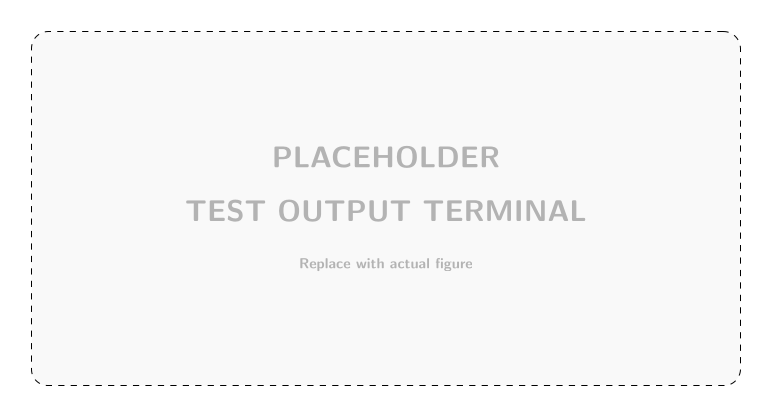
\includegraphics[width=0.85\textwidth]{Images/fig_test_output_terminal.png}
\caption{Terminal output showing all 55 tests passing across the Voting, GN officer/ElectionRegistry, and NicRegistry test suites.}
\label{fig:test-output}
\end{figure}

\begin{table}[H]
\centering
\caption{Test case distribution across contract modules.}
\label{tab:test-distribution}
\begin{tabular}{|l|r|l|}
\hline
\textbf{Test Group} & \textbf{Count} & \textbf{File} \\
\hline
Setup Phase & 8 & Voting.ts \\
\hline
Registration Phase & 10 & Voting.ts \\
\hline
Phase Transitions & 6 & Voting.ts \\
\hline
View Functions & 4 & Voting.ts \\
\hline
Reset / Multi-Election & 9 & Voting.ts \\
\hline
GN Officer Management & 7 & GNAndRegistry.ts \\
\hline
ElectionRegistry & 6 & GNAndRegistry.ts \\
\hline
NicRegistry & 5 & NicRegistry.ts \\
\hline
\textbf{Total} & \textbf{55} & \\
\hline
\end{tabular}
\end{table}

The \texttt{vote()} function's proof-dependent paths are deliberately \emph{not} unit-tested with fabricated proofs---a valid UltraHonk proof cannot be forged inside a test, which is precisely the security property. Instead, the complete vote path (valid proof accepted, wrong root rejected, reused nullifier rejected with \texttt{Voting\_\_NullifierHashAlreadyUsed}) is exercised by the end-to-end pipeline using real proofs generated by the actual prover (Section~\ref{sec:e2e-flow}).

\subsection{Key Test Cases}

\subsubsection{Registration Tests}

\begin{lstlisting}[language=Java, caption={Registration tests: allowlisted voter registers; tree grows with sequential leaf indices.}]
it("allows an allowlisted voter to register a commitment",
  async function () {
    await expect(voting.connect(voter1).register(COMMITMENT_1))
      .to.emit(voting, "NewLeaf")
      .withArgs(0, COMMITMENT_1);
});

it("emits NewLeaf with sequential indices", async function () {
  await expect(voting.connect(voter1).register(COMMITMENT_1))
    .to.emit(voting, "NewLeaf").withArgs(0, COMMITMENT_1);
  await expect(voting.connect(voter2).register(COMMITMENT_2))
    .to.emit(voting, "NewLeaf").withArgs(1, COMMITMENT_2);
});

it("handles multiple registrations and increments depth",
  async function () {
    await voting.connect(voter1).register(COMMITMENT_1);
    await voting.connect(voter2).register(COMMITMENT_2);
    const data = await voting.getVotingData();
    expect(data.depth).to.equal(1n);
});
\end{lstlisting}

\subsubsection{Duplicate-Registration Prevention Tests}

\begin{lstlisting}[language=Java, caption={Test: a NIC hash can be reserved only once, regardless of caller.}]
it("rejects a second reservation of the same hash regardless of caller",
  async function () {
    await registry.connect(gn)
      .reserveNicHash(NIC_HASH, await voting.getAddress());

    await expect(
      registry.reserveNicHash(NIC_HASH, await voting.getAddress())
    ).to.be.revertedWithCustomError(
      registry, "NicRegistry__AlreadyUsed"
    ).withArgs(NIC_HASH);
});
\end{lstlisting}

\subsubsection{Phase Transition Tests}

\begin{lstlisting}[language=Java, caption={Test: automatic phase advancement on deadline expiry.}]
it("auto-advances Registration -> Ended after deadline",
  async function () {
    await ethers.provider.send("evm_increaseTime",
                               [REG_DURATION + 1]);
    await ethers.provider.send("evm_mine", []);
    expect(await voting.currentPhase()).to.equal(Phase.Ended);
});

it("auto-advances Voting -> Ended after deadline",
  async function () {
    await voting.startVoting(VOTE_DURATION);
    await ethers.provider.send("evm_increaseTime",
                               [VOTE_DURATION + 1]);
    await ethers.provider.send("evm_mine", []);
    expect(await voting.currentPhase()).to.equal(Phase.Ended);
});
\end{lstlisting}

\subsubsection{ElectionRegistry Tests}

\begin{lstlisting}[language=Java, caption={Tests: division management and national aggregation.}]
it("returns all divisions", async function () {
  await registry.addDivision("Kaduwela",
    await voting.getAddress(), gn.address);
  await registry.addDivision("Colombo",
    await voting.getAddress(), gn.address);
  const divs = await registry.getAllDivisions();
  expect(divs.length).to.equal(2);
  expect(divs[0].name).to.equal("Kaduwela");
});

it("getNationalVoteCount aggregates across divisions",
  async function () {
    await registry.addDivision("Div1",
      await voting.getAddress(), gn.address);
    await registry.addDivision("Div2",
      await voting.getAddress(), gn.address);
    const count = await registry.getNationalVoteCount(0);
    expect(count).to.equal(0);
});
\end{lstlisting}

\section{Custom Blockchain Verification}\label{sec:chain-verification}

The custom chain's correctness claim---``behaves exactly like an Ethereum node for every operation this system performs''---is established by five complementary mechanisms rather than by trust:

\begin{figure}[H]
\centering
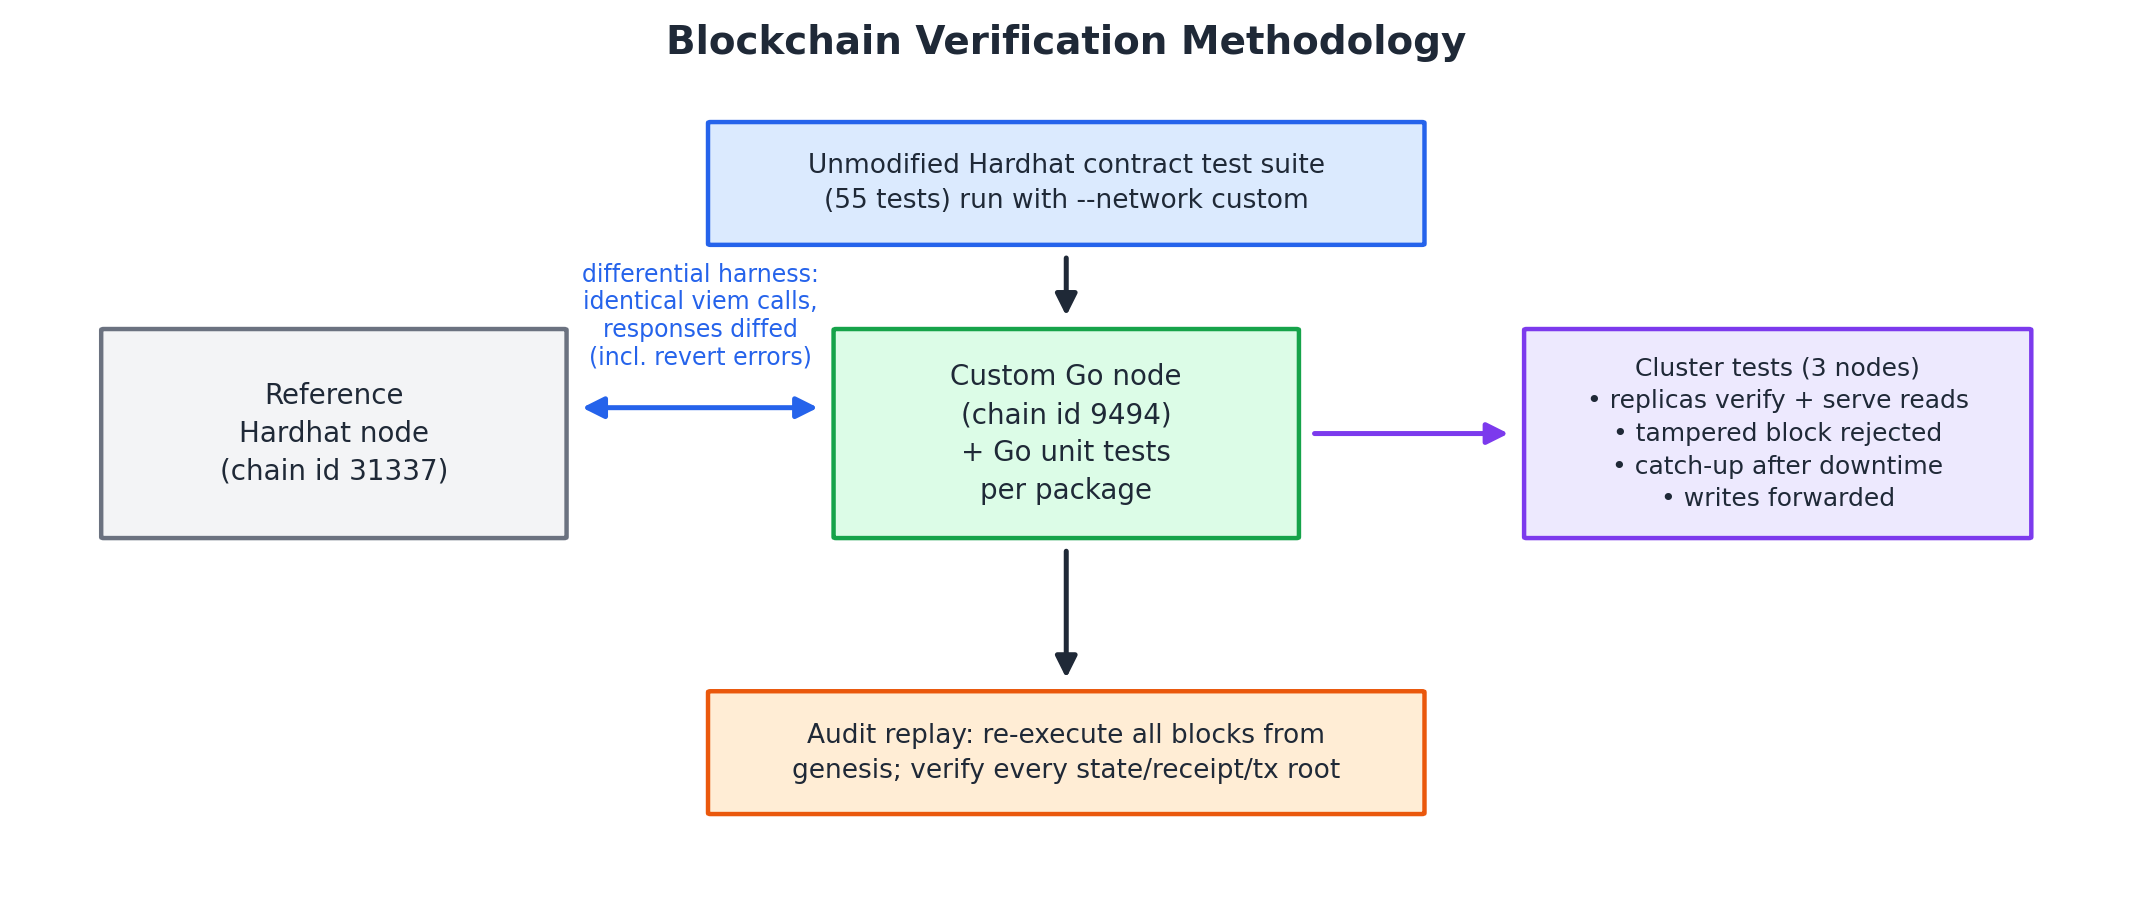
\includegraphics[width=0.92\textwidth]{Images/fig_chain_v2_testing.png}
\caption{Blockchain verification methodology: unit tests, differential testing against a reference Hardhat node, the unmodified contract test suite executed against the Go node, deterministic audit replay, and multi-node replication checks.}
\label{fig:chain-testing}
\end{figure}

\begin{enumerate}
    \item \textbf{Package-level unit tests} (Go) cover configuration validation, genesis determinism, transaction validation (nonce, chain id, gas cap), EVM execution, block sealing, receipt and log derivation, and restart recovery, with table-driven cases per package.
    \item \textbf{Differential testing.} A harness issues identical viem calls to a live Hardhat node and to our node, then diffs the JSON responses after normalizing legitimately volatile fields (hashes, timestamps). This covers read methods, write receipts, and---critically---\emph{error shapes}: a revert with \texttt{Voting\_\_WrongPhase} must decode to the same custom error on both backends, since the applications' error handling depends on it. Response-shape checks additionally run viem's own formatters over the node's JSON to catch field-level deviations.
    \item \textbf{The Hardhat contract suite against the node.} The strongest compatibility evidence: the same 55-test suite from Table~\ref{tab:test-distribution} is executed unmodified with \texttt{--network custom}, so every assertion written for the reference EVM must also hold on ours---including time manipulation via the \texttt{evm\_increaseTime} development methods.
    \item \textbf{Deterministic audit replay.} The standalone audit tool re-executes the full block history on a fresh state database and verifies every block's state root, receipt root, transaction root, and linkage; deliberately corrupted test fixtures are detected at the exact offending block.
    \item \textbf{Replication checks.} Three-node cluster scenarios verify that replicas re-execute and accept honest blocks, reject blocks with tampered state roots, catch up correctly after downtime, and transparently forward writes to the sequencer.
\end{enumerate}

\section{Performance Characteristics}

% TODO(before submission): replace design-derived figures in this section with
% measured values from the blockchain e2e benchmark run (docs/blockchain-v2, M14).

\subsection{Latency Analysis}

\begin{table}[H]
\centering
\caption{Expected operation latency by system layer.}
\label{tab:latency}
\begin{tabular}{|l|l|l|}
\hline
\textbf{Operation} & \textbf{Expected latency} & \textbf{Environment} \\
\hline
Commitment generation & $<$10 ms & Mobile (Poseidon, JS) \\
\hline
Voter registration (tx) & $<$0.5 s & Custom chain (auto-mine) \\
\hline
ZK proof generation & 15--25 s & Mobile WebView (WASM) \\
\hline
Vote transaction (incl.\ on-chain verify) & $<$1 s & Custom chain (EVM Honk verify) \\
\hline
Block finality & Immediate & 1 tx/block, no reorgs \\
\hline
Replica propagation & $<$1 s & mTLS push, LAN \\
\hline
National result query & tens of ms & View call (no gas) \\
\hline
Merkle path retrieval & $<$100 ms & API route over event logs \\
\hline
\end{tabular}
\end{table}

\begin{figure}[H]
\centering
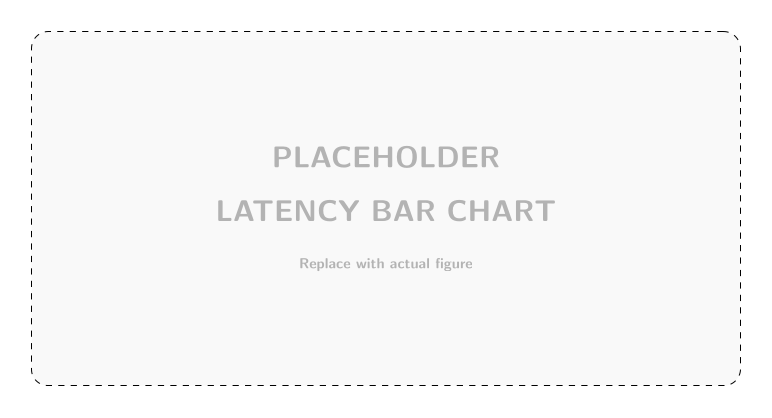
\includegraphics[width=0.85\textwidth]{Images/fig_latency_bar_chart.png}
\caption{Operation latency comparison: proof generation dominates the voter experience at 15--25 seconds; every on-chain step is sub-second.}
\label{fig:latency-chart}
\end{figure}

Because the node auto-mines one transaction per block with instant finality, there is no block-interval waiting time and no confirmation-depth heuristic: a transaction is final the moment its receipt exists.

\subsection{Throughput Analysis}

\begin{figure}[H]
\centering
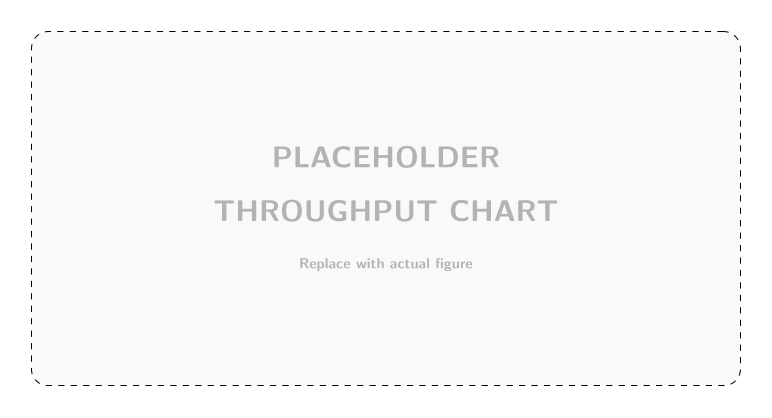
\includegraphics[width=0.85\textwidth]{Images/fig_throughput_chart.png}
\caption{System throughput by operation class: reads scale across replicas; vote throughput is bounded by on-chain proof verification.}
\label{fig:throughput}
\end{figure}

\begin{table}[H]
\centering
\caption{Expected throughput by operation class.}
\label{tab:throughput}
\begin{tabular}{|l|l|l|}
\hline
\textbf{Operation} & \textbf{Expected throughput} & \textbf{Bottleneck} \\
\hline
Registrations & Hundreds of tx/s & LeanIMT Merkle insert \\
\hline
Vote submissions & Tens of tx/s & On-chain Honk verification \\
\hline
Read queries & Thousands of req/s & Scales across read replicas \\
\hline
\end{tabular}
\end{table}

Vote throughput is the binding constraint: each vote executes the full UltraHonk verifier inside the EVM ($\sim$2M gas dominated by BN254 pairing operations), an order of magnitude more compute than any other transaction in the system. The multi-division architecture mitigates this naturally---divisions are independent contracts, and district-level node clusters can operate in parallel (Section~\ref{sec:scalability}).

\section{Gas Analysis}

\subsection{Per-Operation Gas Costs}

% TODO(before submission): replace approximations with the exact hardhat-gas-reporter
% output (packages/hardhat: REPORT_GAS=true yarn test).

\begin{table}[H]
\centering
\caption{Approximate gas consumption per smart contract operation.}
\label{tab:gas-costs}
\begin{tabular}{|l|l|l|}
\hline
\textbf{Operation} & \textbf{Gas (approx.)} & \textbf{Dominant Cost} \\
\hline
\texttt{register()} & 150K--600K & LeanIMT insert (Poseidon per level) \\
\hline
\texttt{vote()} & $\sim$2M & HonkVerifier.verify() pairing check \\
\hline
\texttt{setQuestion()} & $\sim$50K & String storage write \\
\hline
\texttt{setCandidates()} & $\sim$100K & Array storage writes \\
\hline
\texttt{startRegistration()} & $\sim$50K & Phase + deadline write \\
\hline
\texttt{createDivision()} & Several million & Full Voting.sol deployment \\
\hline
\end{tabular}
\end{table}

\texttt{register()} cost grows with tree depth: each LeanIMT insertion recomputes one Poseidon hash per level, so early registrations in a shallow tree are cheaper than late ones at the full depth of 16. The mobile client conservatively reserves 600K gas for registration and 15M for a vote---generous fixed limits chosen because gas is free on the custom chain, making tight estimation pointless.

\begin{figure}[H]
\centering
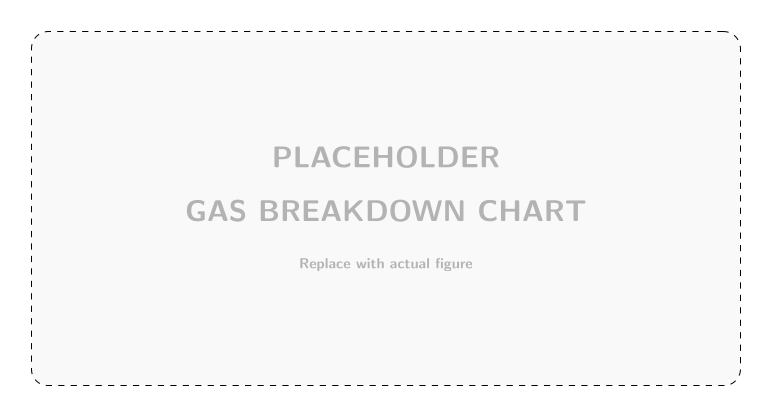
\includegraphics[width=0.85\textwidth]{Images/fig_gas_breakdown_chart.png}
\caption{Gas breakdown for the vote() function: ZK proof verification dominates, with roughly 90\% of the total spent inside HonkVerifier.verify().}
\label{fig:gas-breakdown}
\end{figure}

\subsection{Cost Comparison with Public Chains}

\begin{table}[H]
\centering
\caption{Order-of-magnitude cost if each vote ($\sim$2M gas) were paid at typical public-chain prices; exact figures vary with gas markets and token prices.}
\label{tab:cost-comparison}
\begin{tabular}{|l|l|l|}
\hline
\textbf{Chain} & \textbf{Per Vote} & \textbf{16M Voters} \\
\hline
Ethereum L1 & Tens of USD & Hundreds of millions USD \\
\hline
Optimistic / ZK rollups & \$0.01--\$1 & \$0.2M--\$16M \\
\hline
Polygon PoS & $<$\$0.01 & $<$\$0.2M \\
\hline
Custom chain (ours) & \textbf{\$0.00} & \textbf{\$0} \\
\hline
\end{tabular}
\end{table}

Beyond raw cost, public chains would also require distributing gas tokens to burner wallets---an operational nightmare and a deanonymization vector (the funding trail links a burner to whoever funded it). The gasless custom chain eliminates both problems structurally: a zero-balance burner submits its vote directly.

\section{Security Analysis}

\subsection{Attack-Defense Mapping}

\begin{figure}[H]
\centering
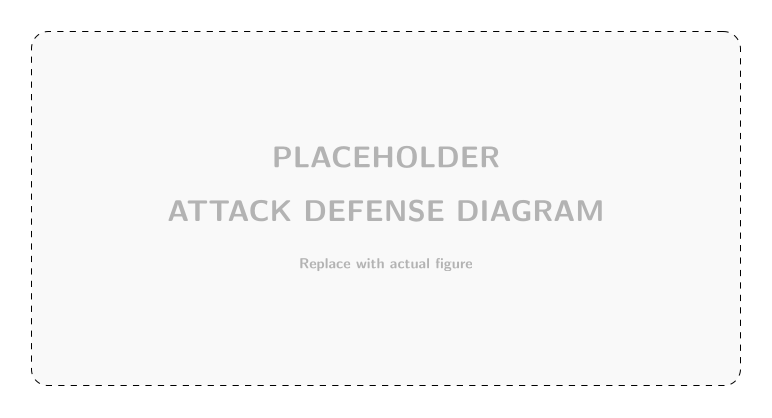
\includegraphics[width=0.85\textwidth]{Images/fig_attack_defense_diagram.png}
\caption{Attack-defense mapping: each potential attack vector and the corresponding defense mechanism.}
\label{fig:attack-defense}
\end{figure}

\begin{table}[H]
\centering
\caption{Security analysis: attack scenarios and defense effectiveness.}
\label{tab:security-analysis}
\resizebox{\textwidth}{!}{%
\begin{tabular}{|p{2.5cm}|p{3cm}|p{3.5cm}|l|p{3cm}|}
\hline
\textbf{Attack} & \textbf{Adversary} & \textbf{Defense} & \textbf{Result} & \textbf{Residual Risk} \\
\hline
Double voting & Voter & Nullifier uniqueness & Prevented & None (deterministic) \\
\hline
Impersonation & External & Biometric + hardware keystore & Prevented & Device theft + biometric \\
\hline
Ballot stuffing & External & ZK proof required & Prevented & None (soundness) \\
\hline
Vote buying & Coercer & Burner wallet & Mitigated & Screenshot before submit \\
\hline
Front-running & Node operator & Vote bound in proof & Prevented & None (cryptographic) \\
\hline
Sybil (multi-div) & Voter & NicRegistry (peppered hash) & Prevented & Fake NIC document \\
\hline
History tampering & Infrastructure & Replica re-execution + audit replay & Detected & Sequencer liveness (censorship is detectable) \\
\hline
Relay compromise & External/insider & Function whitelist + audit log; votes never pass through relay & Bounded & Lifecycle disruption (detectable); cannot forge votes \\
\hline
Admin fraud & Authority & Public verifiability & Detected & N/A (detectable) \\
\hline
Replay attack & External & Nullifier consumed & Prevented & None (one-time) \\
\hline
\end{tabular}%
}
\end{table}

Two rows deserve elaboration. \emph{History tampering}: the single sequencer cannot silently rewrite the record, because every replica re-executes every block and rejects state-root mismatches, and the offline audit tool re-derives the full election from genesis; what remains is a liveness risk (a malicious sequencer could stall or censor), which is externally observable. \emph{Relay compromise}: the administrative relay signs only whitelisted lifecycle functions and structurally cannot sign \texttt{register} or \texttt{vote}, so even full server compromise cannot manufacture or alter a single ballot.

\subsection{Coercion Resistance Analysis}

\begin{figure}[H]
\centering
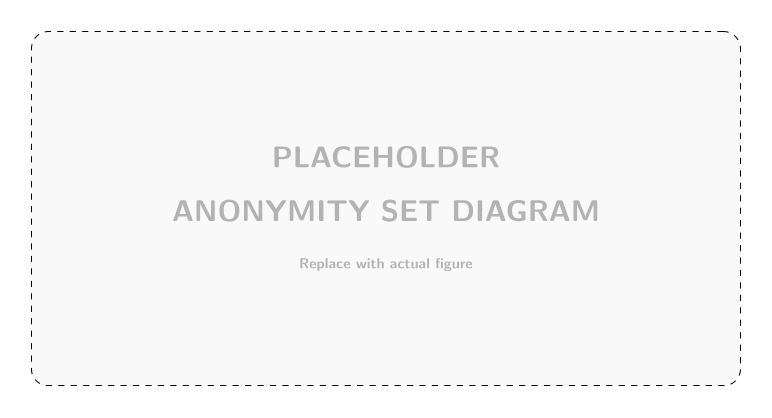
\includegraphics[width=0.85\textwidth]{Images/fig_anonymity_set_diagram.png}
\caption{Anonymity set visualization: a voter's ballot is indistinguishable among all registered voters in the division.}
\label{fig:anonymity-set}
\end{figure}

Our system provides \textbf{partial coercion resistance}:
\begin{itemize}
    \item \textbf{Protected against}: Post-vote coercion (voter cannot prove how they voted after the fact, as the burner wallet is discarded)
    \item \textbf{Vulnerable to}: Real-time coercion (adversary physically present during voting can observe the screen)
    \item \textbf{Mitigation}: The OTP step creates a time window; the actual proof generation and submission can be separated from candidate selection
\end{itemize}

Full coercion resistance would require re-voting capability (as in MACI) or deniable encryption---identified as future work.

\section{Comparison with Existing Systems}

\begin{table}[H]
\centering
\caption{Detailed comparison of our system with MACI, Semaphore, and Voatz.}
\label{tab:system-comparison-detail}
\resizebox{\textwidth}{!}{%
\begin{tabular}{|p{3.5cm}|l|l|l|l|}
\hline
\textbf{Property} & \textbf{Ours} & \textbf{MACI} & \textbf{Semaphore} & \textbf{Voatz} \\
\hline
Proof system & UltraHonk & Groth16 & Groth16 & None \\
\hline
Trusted setup & Universal SRS only & Yes (per-circuit) & Yes (universal) & N/A \\
\hline
Ballot privacy & ZK + burner & Encrypted & ZK proof & Server-side \\
\hline
Trusted coordinator & No & Yes & No & Yes \\
\hline
Gas cost per vote & \$0 (gasless) & $\sim$\$0.50 (L2) & $\sim$\$0.30 (L2) & N/A \\
\hline
Mobile proving & WebView WASM & Not supported & Not supported & N/A \\
\hline
Biometric auth & Hardware TEE & No & No & Central server \\
\hline
Multi-division & 160 divisions & Single election & Single group & Single election \\
\hline
Voter scalability & $\sim$10.5M & $\sim$10K & $\sim$65K & $\sim$1K (tested) \\
\hline
E2E verifiable & Yes & Yes & Partial & No \\
\hline
Double-vote prev. & Nullifier & Nullifier & Nullifier & Server-side \\
\hline
Sybil prevention & Hashed NIC & External & External & ID document \\
\hline
Coercion resistance & Partial & Full (re-vote) & None & None \\
\hline
Open source & Yes & Yes & Yes & No \\
\hline
\end{tabular}%
}
\end{table}

\section{Scalability Analysis}\label{sec:scalability}

\subsection{16 Million Voter Projection}

\begin{figure}[H]
\centering
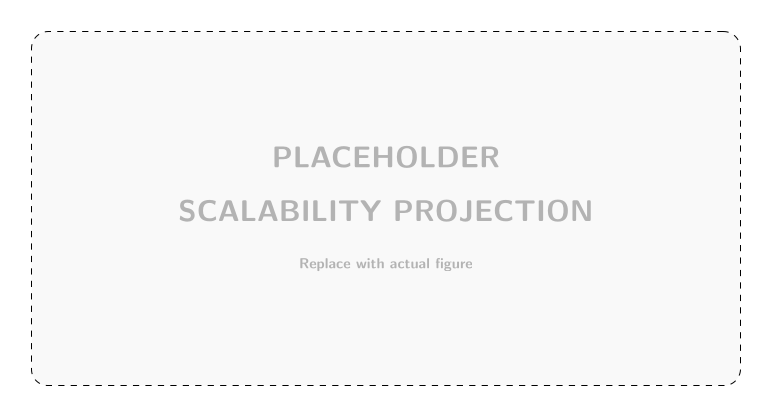
\includegraphics[width=0.85\textwidth]{Images/fig_scalability_projection.png}
\caption{Scalability projection: system capacity for Sri Lanka's 16 million voters across polling divisions.}
\label{fig:scalability}
\end{figure}

\begin{table}[H]
\centering
\caption{Scalability projection for national-scale deployment.}
\label{tab:scalability}
\begin{tabular}{|l|r|l|}
\hline
\textbf{Metric} & \textbf{Value} & \textbf{Calculation} \\
\hline
Total voters & 16,000,000 & Sri Lanka registered voters \\
\hline
Max voters per division & 65,536 & $2^{16}$ (fixed circuit depth of 16) \\
\hline
Capacity at 160 divisions & 10,485,760 & $160 \times 65{,}536$ \\
\hline
Divisions for 16M voters & 245 & $\lceil 16\text{M} / 65{,}536 \rceil$ \\
\hline
Voting window & 12 hours & Typical election day \\
\hline
Required national rate & $\sim$370 votes/sec & 16M / 43,200 s \\
\hline
Single-cluster vote rate & Tens/sec & On-chain Honk verification \\
\hline
\end{tabular}
\end{table}

The circuit never needs modification: capacity scales by \emph{adding divisions}, not by deepening the tree. The gap between the required national rate and a single cluster's vote throughput is closed by parallelism, which the architecture provides for free---divisions are fully independent contracts, so district-level chain clusters (each a sequencer with replicas, carrying a subset of divisions) can process votes concurrently, with the registry aggregation performed off-chain across clusters. Complementary future optimizations include proof batching and recursive aggregation (Chapter~\ref{ch:conclusion}).

\subsection{Storage Requirements}

\begin{table}[H]
\centering
\caption{Approximate storage requirements for a national-scale election.}
\label{tab:storage}
\begin{tabular}{|l|l|l|}
\hline
\textbf{Data} & \textbf{Per Item} & \textbf{16M Voters} \\
\hline
Commitments (Merkle leaves) & 32 bytes & 512 MB \\
\hline
Nullifier hashes & 32 bytes & 512 MB \\
\hline
Vote proofs (tx calldata) & $\sim$14 KB & $\sim$220 GB \\
\hline
Vote counts & 32 bytes/candidate & Negligible \\
\hline
Block overhead (headers, receipts) & $\sim$1 KB/block & $\sim$32 GB \\
\hline
\textbf{Total (order of magnitude)} & & $\sim$250 GB \\
\hline
\end{tabular}
\end{table}

The UltraHonk proof ($\sim$14~KB of calldata per vote) dominates storage. This is well within commodity-server capacity for a national election, and is naturally partitioned across district clusters. Proofs are verified at ingest---they are retained only to keep the full history independently re-executable by the audit tool.

\section{Circuit Correctness Verification}

\subsection{Test Vector Validation}

We generated deterministic test vectors and verified consistency across all system layers: the same input hashed by \texttt{poseidon-lite} in the browser/mobile JavaScript, by the Noir standard library's BN254 Poseidon inside the circuit, and by the \texttt{PoseidonT3} library on-chain must produce the identical field element.

\begin{table}[H]
\centering
\caption{Cross-layer test vector verification.}
\label{tab:test-vectors}
\begin{tabular}{|l|l|l|}
\hline
\textbf{Layer} & \textbf{Implementation} & \textbf{Result} \\
\hline
Browser / mobile & poseidon-lite (JS) & identical field element \\
\hline
Circuit & Noir stdlib \texttt{bn254::hash} & identical field element \\
\hline
On-chain & PoseidonT3 (Solidity) & identical field element \\
\hline
\end{tabular}
\end{table}

All three layers agree on every tested vector, confirming Poseidon parameterization consistency---a critical requirement that took three days to debug during development (see Chapter~\ref{ch:methodology}).

\section{End-to-End Flow Validation}\label{sec:e2e-flow}

The complete flow was validated repeatedly across backends: GN enrolls a voter (NIC hash reservation + allowlisting), the voter registers a commitment from the mobile app (OTP + biometric), generates a real UltraHonk proof in the WebView prover, and casts an anonymous vote from a fresh burner; results update live on the web dashboards, and the voter confirms inclusion via the nullifier-based ``Verify My Vote'' screen. Negative paths are asserted in the same runs: a second vote with the same nullifier is rejected with \texttt{Voting\_\_NullifierHashAlreadyUsed}, a stale Merkle root with \texttt{Voting\_\_InvalidRoot}, and out-of-phase actions with \texttt{Voting\_\_WrongPhase}. On the custom chain the same flow additionally proves the gasless property (the burner holds zero balance) and survives a node restart with full state recovery.

\section{Observations and Discussion}

\subsection{Proof Generation Time}

The 15--25 second proof generation time on mobile is the primary user experience bottleneck. While acceptable for a once-per-election action, this could be reduced to $<$5 seconds with native proving (Swoir/noir\_android)---identified as future work.

\subsection{Hermes Compatibility Trade-offs}

The Hermes BigInt limitation forced a WebView-based architecture for proof generation. While this adds complexity, it provides a clean separation between the UI layer (Hermes) and the cryptographic layer (system WebView with full BigInt support).

\subsection{Gas Efficiency}

The vote function's cost is dominated by proof verification: roughly 90\% of its $\sim$2M gas is spent inside \texttt{HonkVerifier.verify()} on BN254 pairing operations. On our gasless chain this cost is free to the voter but still bounds throughput. For any future public-L2 deployment it could be reduced by:
\begin{itemize}
    \item Batch verification (multiple proofs in one pairing check)
    \item Recursive proofs (aggregate many votes into one proof)
    \item Optimized verifier circuits
\end{itemize}

\subsection{Multi-Division Trade-offs}

The factory pattern provides excellent isolation and administrative delegation but introduces aggregation overhead: \texttt{getNationalResults()} iterates across all divisions, an $O(n)$ view call. For 160 divisions this is negligible (view calls are free and the results API caches them), but a deployment with thousands of divisions would move aggregation off-chain entirely.

\section{Summary}

Our comprehensive evaluation demonstrates:
\begin{enumerate}
    \item \textbf{Correctness}: All 55 contract unit tests pass---on the reference Hardhat network \emph{and} unmodified against the custom Go chain; cross-layer test vectors verify cryptographic consistency
    \item \textbf{Compatibility}: Differential testing shows the custom chain is JSON-RPC-indistinguishable from an Ethereum node for every operation the system performs
    \item \textbf{Performance}: Vote submission completes in $<$30 seconds end-to-end, dominated by mobile proof generation; on-chain steps are sub-second with instant finality
    \item \textbf{Security}: All identified attack vectors are either prevented cryptographically or rendered detectable through replication and audit replay
    \item \textbf{Scalability}: 10.5M voters at 160 divisions with no circuit modification; national scale reached by adding divisions and parallel district clusters
    \item \textbf{Cost}: Zero gas fees for voters (gasless chain), removing both the economic barrier and the funding-trail deanonymization vector
    \item \textbf{Privacy}: Formal voter--ballot unlinkability (Theorem~\ref{thm:unlinkability})
\end{enumerate}

\begin{figure}[H]
\centering
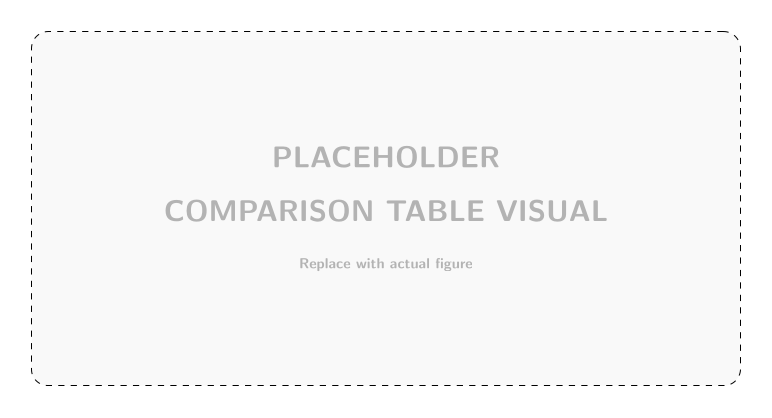
\includegraphics[width=0.85\textwidth]{Images/fig_comparison_table_visual.png}
\caption{Visual comparison summary: our system achieves the best combination of privacy, cost, and scalability among evaluated systems.}
\label{fig:comparison-visual}
\end{figure}

The system successfully demonstrates that privacy-preserving blockchain voting is feasible with current technology, though production deployment would require addressing the limitations identified in Chapter~\ref{ch:conclusion}.
